% IEEE Access working article. Author and archive placeholders require completion.
\let\OriginalTeXYear\year
\PassOptionsToClass{journal,twocolumn}{IEEEtran}
\documentclass[nolineno]{ieeeaccess}
\let\AccessPublicationYear\year
\let\year\OriginalTeXYear
\vol{[UNASSIGNED]}\AccessPublicationYear{[UNASSIGNED]}
\setlength{\paperwidth}{203.2mm}\setlength{\paperheight}{276.2mm}
\AddToHook{shipout/background}{\special{papersize=203.2mm,276.2mm}}
\newif\ifAccess\Accesstrue
\usepackage[T1]{fontenc}
\usepackage{cite,amsmath,amssymb,graphicx,booktabs,tabularx,array,xurl,tikz}
\usetikzlibrary{positioning,arrows.meta}
\usepackage{algorithm,algpseudocode}
\ifAccess
\else
\usepackage{newtxtext,newtxmath}
\usepackage[hidelinks]{hyperref}
\fi
\definecolor{navy}{HTML}{203C55}
\definecolor{teal}{HTML}{167F82}
\setlength{\emergencystretch}{1.2em}
\newcolumntype{Y}{>{\raggedright\arraybackslash}X}
\renewcommand{\tabularxcolumn}[1]{p{#1}}
\setlength{\textfloatsep}{12pt plus 2pt minus 2pt}
\setlength{\dbltextfloatsep}{12pt plus 2pt minus 2pt}
\setlength{\floatsep}{10pt plus 2pt minus 2pt}
\setlength{\dblfloatsep}{10pt plus 2pt minus 2pt}
\renewcommand{\arraystretch}{1.15}
% Keep the body in two columns even when an editor changes class defaults.
\makeatletter
\AtBeginDocument{\if@twocolumn\else\twocolumn\fi
\typeout{APISHIELD-LAYOUT: two-column body; column=\the\columnwidth; text=\the\textwidth}}
\makeatother
\widowpenalty=10000\clubpenalty=10000

% Access's bundled Type 1 fonts need their map files under XeTeX/Tectonic.
\ifdefined\XeTeXversion
\special{pdf:mapfile t1-times.map}
\special{pdf:mapfile t1-formata.map}
\special{pdf:mapfile t1-giovannistd.map}
\fi
\makeatletter
\AtBeginDocument{\DeclareMathVersion{bold}
\SetSymbolFont{operators}{bold}{T1}{times}{b}{n}
\SetSymbolFont{NewLetters}{bold}{T1}{times}{b}{it}
\SetMathAlphabet{\mathrm}{bold}{T1}{times}{b}{n}
\SetMathAlphabet{\mathit}{bold}{T1}{times}{b}{it}
\SetMathAlphabet{\mathbf}{bold}{T1}{times}{b}{n}
\SetSymbolFont{symbols}{bold}{OMS}{cmsy}{b}{n}}
\makeatother
\begin{document}
\history{Working manuscript for author review.}
\doi{}
\title{APIShield: Behavioral Preservation in REST API Migration Through Semantic Context and Inferred Checks}
\author{Dr. Anusha K, Surjith Khannan, Sadhana S, AND Mohammed Ashfaque}
\markboth{Anusha K et al.: APIShield}{Anusha K et al.: APIShield}
\begin{abstract}
Client code can satisfy a revised REST API schema while changing an exact monetary amount, destination or idempotency key. APIShield addresses this migration problem by connecting contract differences to source context and executable preservation checks. A Semantic Intent Graph distinguishes observed source relationships from inferred behavioral interpretations. A bounded repair loop uses public tests and inferred checks, while a separate hidden oracle evaluates the selected candidate. We analyze an author-supplied release of 720 treatment records over 120 curated Python migration tasks. Six configurations separate structural and semantic context from test-only and inferred-check validation. The full configuration achieves 80.8\% hidden correctness, compared with 28.3\% for iterative test feedback. The paired gain is 52.5 percentage points, with a 95\% domain-stratified bootstrap interval of 42.5--62.5. Across 60 financial tasks, joint invariant preservation is 86.7\% versus 31.7\%. Estimated API cost per hidden-correct repair decreases by 33.5\%, although expenditure per task increases. Factorial contrasts indicate overlapping component benefits, and the structural-context configuration with inferred checks has the lowest cost per correct result. The article develops the acceptance model, examines assertion coverage through a retained failure case, and specifies the limits and reproduction requirements of the curated evaluation.
\end{abstract}
\begin{keywords}
API evolution, automated program repair, behavioral preservation, empirical software engineering, large language models, OpenAPI, semantic intent graphs.
\end{keywords}
\titlepgskip=-15pt
\newlength{\savedparagraphindent}\setlength{\savedparagraphindent}{\parindent}
\setlength{\parindent}{0pt}\maketitle\setlength{\parindent}{\savedparagraphindent}
\section{Introduction}
A client can conform to a revised REST interface and still perform the wrong operation. Moving a payment amount into a nested object preserves the request shape only if its monetary unit and exact value also survive the edit. An idempotency token can be syntactically optional yet necessary to prevent duplicate operations. These obligations make API migration a maintenance problem that extends beyond schema compatibility.

OpenAPI descriptions expose operations and data structures in a form that tools can compare~\cite{openapi}. They rarely provide a complete executable specification of a consuming application's business behavior. A migration assistant must connect the provider's change to client code, identify behavior that should remain stable, and produce a patch whose acceptance has an inspectable basis. Patch-plausibility research shows why available tests alone may be insufficient: a candidate can satisfy them while changing untested behavior~\cite{plausibility2015}.

APIShield addresses this problem for supported Python REST integrations. It relates versioned contracts to source-level call sites, enriches the selected context with inferred intent, and evaluates proposed edits against public tests and additional executable checks. A Semantic Intent Graph (SIG) represents source relationships together with declared or inferred behavioral interpretations. Generated checks guide the repair loop. A separate hidden oracle assesses the retained candidate after that loop ends. The resulting patch remains subject to developer review.

The research question is whether the additional context and checks improve independently assessed migration outcomes enough to justify their inference cost. The evaluation covers 120 curated migration tasks and six treatments, yielding 720 task-level records. The full configuration passes the hidden evaluator on 97 tasks, compared with 34 for iterative test feedback. Pairing the treatments on the same tasks separates the effect of the repair configuration from differences in task composition.

The study examines how semantic context and executable preservation checks work together during REST migration. It defines the repair boundary, evaluates the two mechanisms through a six-treatment design, and relates hidden correctness to localization, financial obligations and inference cost. The comparison tests their combination; repository graphs and invariant inference have established precedents.

\ifAccess
\subsection{Scope and intended use}
The target user maintains a trusted local repository and has access to previous and updated API descriptions. APIShield helps prepare a reviewable migration proposal. Its Python engine is shared by a command-line interface and a browser workspace coordinated through FastAPI. The browser presents contracts, source relationships, proposed edits and validation evidence. Interface behavior is separate from the benchmark's unit of evaluation.

The research task is smaller than a deployed integration. A fixture exposes a Python request builder and explicit input/output behavior. This supports controlled comparisons of candidate construction and preservation checks. Claims about distributed retries, concurrent settlements, production authentication or human review effort require other observations. Preserving an idempotency field in a request is an observable obligation; exactly-once execution of a remote transaction is a system-level property.

We distinguish three sources of evidence throughout the article. Static analysis establishes supported source relationships. Inferred rules propose behavior to check. Independent evaluator assertions assess selected outputs. Keeping these sources visible prevents a model explanation, a passing generated test and a hidden-oracle result from being treated as equivalent evidence.
\fi

\section{Background and Related Work}
\subsection{API evolution and migration repair}
APIDiff identifies breaking and non-breaking changes between Java library versions~\cite{apidiff2018}. APIfix uses output-oriented synthesis to adapt clients after library changes~\cite{apifix2021}; ASAP-Repair uses API usage graphs for API-specific repair~\cite{asap2024}. These systems establish precedents for connecting API changes with client edits. Their library interfaces and datasets differ from versioned REST contracts, so their published success rates are not direct baselines for this benchmark.

For REST clients, dcFix combines specification-based identification of non-conforming fragments with LLM repair~\cite{dcfix2025}. APIShield examines a related setting in which an old contract, a new contract and preservation obligations jointly constrain a migration. Its proposed distinction is the experimental combination of contextual representation and additional behavioral checks. A direct comparison with dcFix would require a common implementation, task population and budget; the present experiment compares the six APIShield configurations.

\subsection{LLM repair and repository context}
ChatRepair studies conversational repair using feedback from earlier candidates~\cite{chatrepair2024}. RepairAgent provides a tool-using LLM workflow~\cite{repairagent2024}, while SWE-bench supplies repository-level tasks derived from GitHub issues~\cite{swebench2024}. These studies motivate iterative generation and reproducible task descriptions, but differ from the compact migration fixtures used here.

RepoGraph provides repository-level graph context for software-engineering agents~\cite{repograph2025}. SpecRover investigates intent extraction and specification inference during repair~\cite{specrover2024}. APIShield applies related ideas to relationships between a changed remote operation and client behavior. Static edges and inferred interpretations remain distinguishable, because a correct source relationship does not establish that its inferred business meaning is correct.

\subsection{Invariants and service testing}
Daikon demonstrates inference of likely invariants from execution observations~\cite{daikon2007}. Such invariants are hypotheses whose usefulness depends on their supporting observations. In APIShield, inferred intent supplies candidate checks whose assertions still need independent evaluation.

RESTler generates stateful API tests from service descriptions and execution feedback~\cite{restler2019}. RestSpecIt uses LLM-assisted request mutations for REST documentation and testing~\cite{restspecit2025}. These approaches primarily exercise service behavior. APIShield's repair target is the consuming client's source. Service testing could strengthen migration validation, but its results cannot substitute for the client-side hidden-oracle endpoint.

\ifAccess
\subsection{Position of the present comparison}
Dependency migration can require coordinated edits beyond one call. Fruntke and Krinke study repair of dependency-breaking changes~\cite{dependency2025}, illustrating that broader maintenance setting. We isolate request-builder changes so that exact obligations can be stated and identical tasks compared across treatments. This improves interpretability while restricting external validity.

Public tests participate in candidate selection. Repeated optimization can exploit their omissions, which motivates a held-out evaluator~\cite{plausibility2015}. Generated checks occupy a third position: they are intentionally visible and can improve selection, but cannot also serve as the independent endpoint used to claim correctness. This separation is central to the experimental design.

Differences in models, tasks, context and budgets prevent a numerical ranking against published success rates. The quantitative comparisons use treatments evaluated on the same task identifiers.
\fi

\section{Problem Definition and Evidence Model}
Let $P$ be a client at revision $r$, and let $C_o,C_n$ be its previous and updated contracts. A task supplies an allowed edit region $A$, public tests $T_v$, and application obligations $R$. A patch $\pi$ produces $P'=\pi(P)$. A useful migration satisfies the updated interface while preserving obligations applicable to the affected operation.

We express operational acceptance as
\begin{equation}
\mathcal A(\pi)=S(\pi,A)\land T_v(P')\land T_g(P',R),
\label{eq:accept}
\end{equation}
where $S$ checks syntax, permitted files and edit integrity, and $T_g$ denotes applicable generated or confirmed requirement checks. This rule summarizes available evidence. It does not imply universal semantic equivalence between $P$ and $P'$.

Independent evaluation uses a different suite $T_h$, applied only after selection. We define $Y_{tm}=1$ when task $t$ under method $m$ satisfies that hidden evaluator. Unsuccessful tasks remain in the denominator. Public and hidden passage are distinct outcomes. When a needed field cannot be recovered from available inputs, an actionable diagnostic may be more appropriate than an invented default.

\ifAccess
\subsection{Relational preservation obligations}
An obligation identifies a source scope, a behavioral statement and the evidence used to check it. Monetary preservation can require an integer minor-unit amount equal to the caller's input. Routing preservation relates an input destination to the destination sent in the request. Idempotency preservation relates the caller's key to the outgoing header. These are relations over inputs and outputs, not simply tests for field presence.

Representative predicates for an amount and key are
\begin{align}
R_a(d,o)&:\;\operatorname{type}(o.a)=\mathrm{int}\land o.a=d.a,\\
R_k(d,o)&:\;o.k=d.k,
\end{align}
where $d$ is an evaluator input and $o$ the constructed request. Field paths depend on the updated contract. A type assertion alone does not establish equality, and a present header does not establish preservation of its value.

An inferred obligation can preserve a pre-existing bug. Developer confirmation and independent assertions address different parts of that problem. Confirmation records the requirement accepted by the developer. An oracle checks its selected behavioral consequences. Neither establishes that the specification is complete.

\subsection{Evidence identities}
A run associates source and contract identities with treatment, prompts, candidates and validation outputs. This lets reviewers distinguish the edit that was tested from a later edit with similar text. The retained patch should be derived from checked source bytes. Changes to source, tests or requirement definitions create a new evaluation context even when the task identifier stays the same.

The quantitative analysis uses the supplied evaluation release. Reproducible publication requires a frozen version in which run-time source, inferred checks and original responses correspond to the reported outputs. A checksum establishes a file's byte identity; it does not independently establish its execution history.
\fi

\section{APIShield Method}
\subsection{Contract comparison and impact scope}
APIShield captures selected source and compares the supplied OpenAPI versions. The implementation uses oasdiff for contract-level changes~\cite{oasdiff}. A conservative Python scanner recovers supported direct HTTP calls and surrounding functions. Unresolved targets remain explicit limitations of the analysis rather than silently becoming unaffected code.

The impact scope connects changed operations with consuming functions. Structural context contains observed source relationships; semantic context adds interpretations of the operations and their values. The research harness implements a compact representation for request-builder fixtures. The browser can display a broader repository graph, whose whole-repository scalability is not measured by this experiment.

\subsection{Semantic Intent Graph}
Write the SIG as $G=(V,E_s,E_i)$, with source and operation nodes $V$, observed structural edges $E_s$, and declared or inferred intent edges $E_i$. Edges retain their origin. A payload field can be related to a caller input and an obligation to preserve its unit, while a separate edge identifies the function issuing the changed request.

The graph selects context relevant to the changed operation and explains why each source region or obligation was included (Fig.~\ref{fig:sig}). Structural edges record observed relationships; intent edges retain their declared or inferred origin. An inferred interpretation remains a hypothesis until its behavioral consequences are checked.

\begin{figure*}[t]
\centering
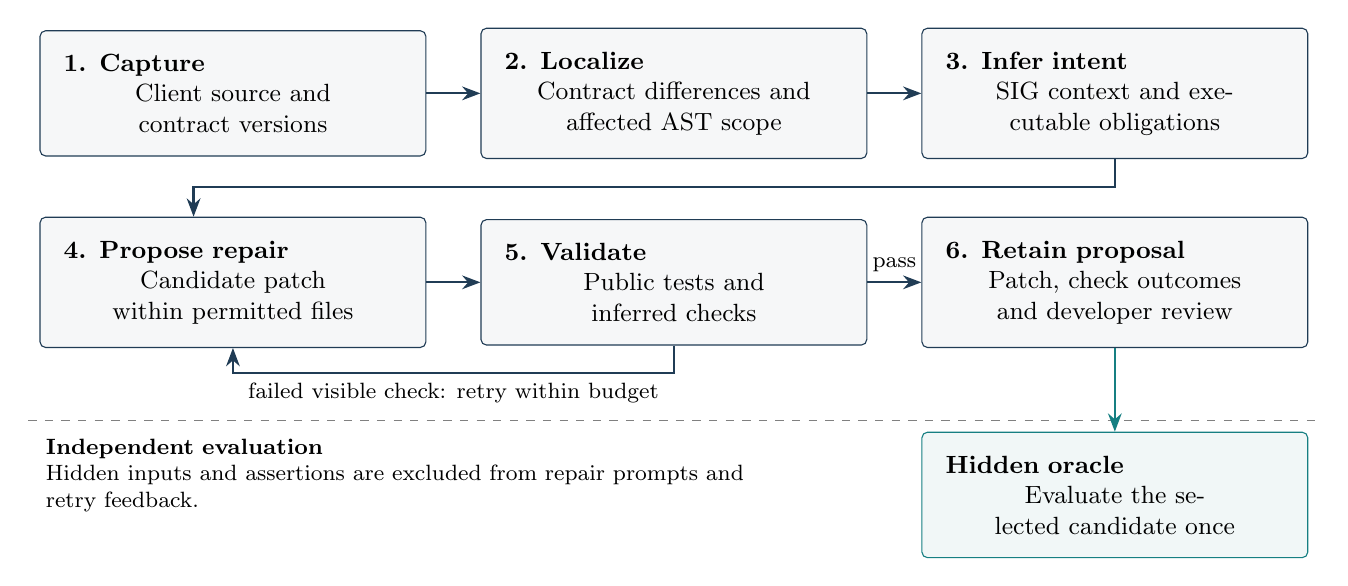
\begin{tikzpicture}[>=Stealth,
box/.style={draw=navy,rounded corners=2pt,fill=navy!4,align=center,font=\small,text width=43mm,minimum height=14mm,inner sep=3mm},
arr/.style={->,thick,draw=navy},note/.style={font=\footnotesize,align=center}]
\node[box](source)at(0,0){\textbf{1. Capture}\newline Client source and contract versions};
\node[box](impact)at(5.6,0){\textbf{2. Localize}\newline Contract differences and affected AST scope};
\node[box](intent)at(11.2,0){\textbf{3. Infer intent}\newline SIG context and executable obligations};
\node[box](generate)at(0,-2.4){\textbf{4. Propose repair}\newline Candidate patch within permitted files};
\node[box](validate)at(5.6,-2.4){\textbf{5. Validate}\newline Public tests and inferred checks};
\node[box](retain)at(11.2,-2.4){\textbf{6. Retain proposal}\newline Patch, check outcomes and developer review};
\draw[arr](source)--(impact);\draw[arr](impact)--(intent);
\draw[arr](intent.south)--++(0,-.35)-|([xshift=-5mm]generate.north);
\draw[arr](generate)--(validate);\draw[arr](validate)--node[above,note]{pass}(retain);
\draw[arr](validate.south)--++(0,-.35)-|node[pos=.25,below,note]{failed visible check: retry within budget}(generate.south);
\draw[dashed,gray](-2.6,-4.15)--(13.8,-4.15);
\node[note,anchor=west,text width=95mm,align=left]at(-2.5,-4.85){\textbf{Independent evaluation}\newline Hidden inputs and assertions are excluded from repair prompts and retry feedback.};
\node[box,draw=teal,fill=teal!6](oracle)at(11.2,-5.1){\textbf{Hidden oracle}\newline Evaluate the selected candidate once};
\draw[arr,draw=teal](retain)--(oracle);
\end{tikzpicture}
\caption{APIShield architecture and evaluation boundary. The repair loop uses visible feedback. The evaluator receives the selected candidate after the loop ends.}\label{fig:architecture}
\end{figure*}

\subsection{Intent extraction and executable checks}
Intent inference proposes bounded statements and executable checks for the affected scope. The application distinguishes inferred rules from developer-confirmed requirements. Generated tests use a separate location, and existing repository tests are protected from replacement. The assistant therefore cannot satisfy validation by weakening the original suite.

A generated check can reject a migration that ordinary regression tests overlook. Its adequacy remains a separate concern. A shape assertion may miss the exact amount, destination or token. We retain individual outcomes and use independently authored hidden assertions for the quantitative endpoint. Passing the generated suite establishes only that suite's assertions on its selected inputs.

\subsection{Bounded repair and acceptance}
The engine creates a disposable workspace from the captured baseline. An attempt proposes an edit within permitted files, validates structure and runs public tests and applicable requirement checks. Failed visible checks can enter a later prompt. Hidden assertions and outputs stay outside the retry context. The loop terminates with an accepted proposal, failure, or request for missing information.

Accepted candidates remain reviewable patches. Application to working source requires freshness and integrity checks. Publication through a draft-pull-request workflow is a separate explicit action. The benchmark measures candidate behavior rather than production deployment or acceptance by maintainers.

\subsection{Repair procedure and outcome states}
Algorithm~\ref{alg:repair} summarizes the control boundary. Public tests and generated checks are evaluated separately because they answer different questions. A failed visible check can trigger another attempt. An unresolved requirement or missing input can terminate without an edit. A scan with no detected impact is also a distinct outcome; it does not count as a repaired migration.

\begin{algorithm}[t]
\caption{Bounded repair and final-only independent evaluation}\label{alg:repair}
\begin{algorithmic}[1]
\Require $P,C_o,C_n$, edit region $A$, tests $T_v$, budget $K$
\State $D\gets\operatorname{Diff}(C_o,C_n)$
\State $G\gets\operatorname{Context}(P,D)$
\State $R,T_g\gets\operatorname{InferOrConfirm}(P,D,G)$
\For{$j=1,\ldots,K$}
 \State $W\gets\operatorname{FreshCopy}(P)$
 \State $\pi\gets\operatorname{Generate}(W,D,G,R,\text{visible feedback})$
 \If{required information is unavailable}
  \State \Return missing-information diagnostic
 \EndIf
 \If{$S(\pi,A)\land T_v(\pi(W))\land T_g(\pi(W),R)$}
  \State retain candidate and evidence; end repair loop
  \State apply $T_h$ once for independent evaluation
  \State \Return patch and separate evaluator outcome
 \EndIf
 \State update feedback from visible checks only
\EndFor
\State \Return unsuccessful repair with retained evidence
\end{algorithmic}
\end{algorithm}

The product also distinguishes cancellation, provider failure and stale-source rejection. These states affect end-to-end availability. Asking whether a model can construct a correct patch differs from asking whether an application delivered a proposal despite infrastructure failures. Evaluation denominators must state which population they describe.

\subsection{Implementation boundary}
The Python engine coordinates source capture, comparison, generation, edit validation and durable records. FastAPI exposes this workflow to the React workspace. The CLI and browser share the engine, so acceptance does not depend on browser-only checks. Repository commands execute trusted local code. A temporary directory protects the original checkout from accidental writes, but is not an operating-system sandbox.

The primary evaluation executes trusted fixtures. Temporary workspaces separate edits from the original source; they do not provide operating-system isolation. The accounting endpoint is API usage.

\begin{figure}[t]\centering
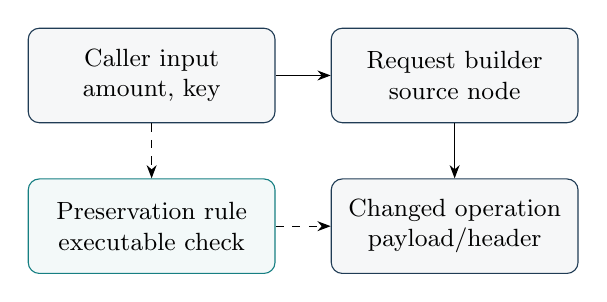
\begin{tikzpicture}[>=Stealth,n/.style={draw=navy,fill=navy!4,rounded corners,align=center,font=\small,text width=29mm,minimum height=12mm},node distance=7mm]
\node[n](i){Caller input\\amount, key};\node[n,right=of i](s){Request builder\\source node};
\node[n,below=of s](o){Changed operation\\payload/header};\node[n,left=of o,draw=teal,fill=teal!5](r){Preservation rule\\executable check};
\draw[->](i)--(s);\draw[->](s)--(o);\draw[->,dashed](i)--(r);\draw[->,dashed](r)--(o);
\end{tikzpicture}
\caption{Conceptual SIG fragment. Solid edges denote observed structure; dashed edges denote declared or inferred preservation relationships.}\label{fig:sig}
\end{figure}

\ifAccess
\subsection{Bounded model interaction}
The application's intent interface constrains both the form and size of an inference response. Rules must identify a known Python source file and function. Their origin remains AI-inferred until a developer adopts and confirms a definition. Generated checks must use distinct test paths and cannot overwrite existing files. These checks make an answer structurally usable; they do not establish the truth of the inferred requirement.

The current interface permits at most 16 rule descriptions and between one and 12 check files, with a 32 KiB aggregate generated-code limit. Rule descriptions are bounded to 800 characters. The request-builder harness uses a separate compact response schema. These application limits constrain response admission; their optimal values are not tested here.

Validation also distinguishes source admissibility from behavioral adequacy. Parsing a check, resolving its referenced scope and rejecting unknown names can prevent malformed test code from entering validation. A syntactically valid assertion can still be vacuous or test the wrong relation. The separate private oracle is consequently needed even after response validation succeeds.

\begin{table}[t]\centering\small
\caption{Distinct validation responsibilities in the application and benchmark.}\label{tab:boundaries}
\begin{tabularx}{\columnwidth}{@{}lXX@{}}\toprule
Boundary & What it establishes & What remains open\\\midrule
Response schema & Required fields and bounded output & Whether inferred intent is correct\\
Scope checks & Known source/function and allowed paths & Whether all affected code was found\\
Public tests & Available regression assertions pass & Unasserted behavioral obligations\\
Generated checks & Inferred assertions pass & Assertion completeness and accuracy\\
Hidden oracle & Private assertions pass on held-out inputs & General correctness and deployed behavior\\\bottomrule
\end{tabularx}
\end{table}

When the attempt budget is exhausted, the engine retains the failed candidate and its visible outcomes. The record distinguishes missing inputs, unsupported analysis, provider errors and unsuccessful edits. Table~\ref{tab:boundaries} identifies the validation boundary associated with each result; diagnostic accuracy is outside the measured endpoints.

\subsection{Review interface}
The review workspace separates ordinary tests from inferred rules and exposes each outcome beside the candidate (Fig.~\ref{fig:interface}). Developers can inspect the proposed edit and its supporting checks before applying it. This interface capture documents the application workflow; benchmark outcomes come from the separate evaluator.

\begin{figure*}[t]\centering
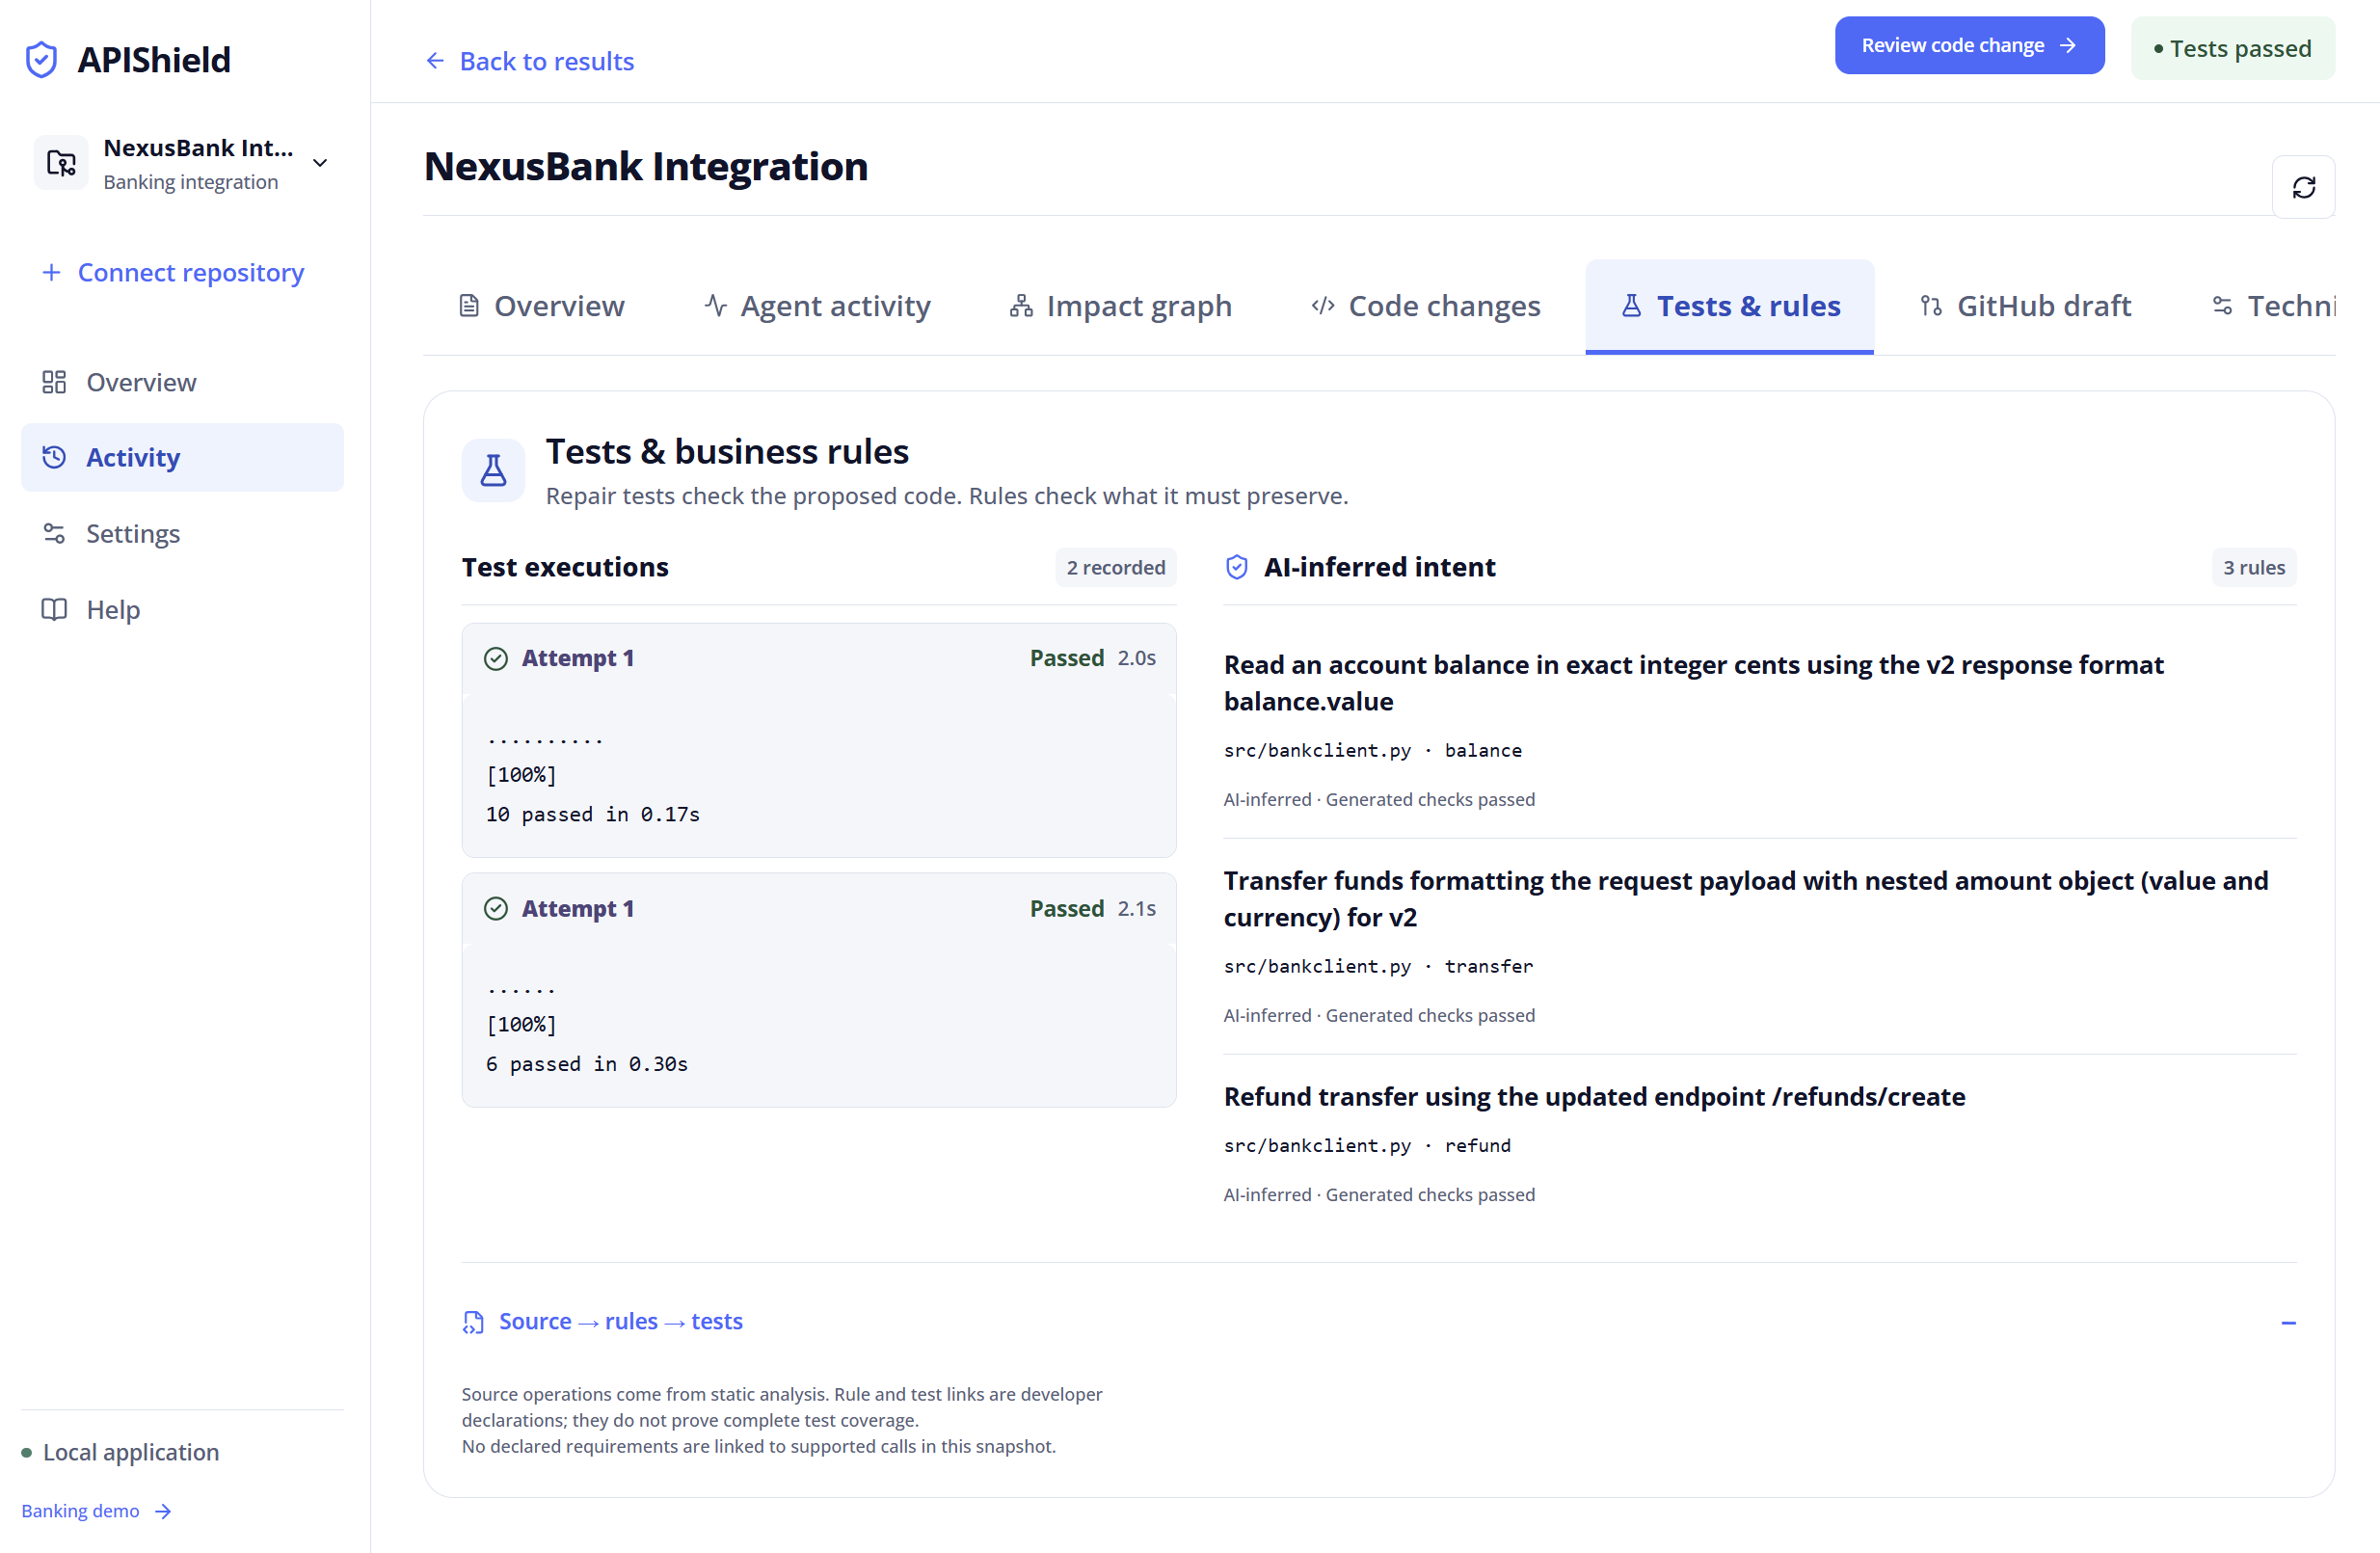
\includegraphics[width=.76\textwidth,trim=290bp 0 0 0,clip]{figures/review_interface.png}
\caption{Implemented review interface showing tests and inferred rules. The quantitative analysis uses the separate benchmark release, not this application capture.}\label{fig:interface}
\end{figure*}
\fi

\section{Benchmark and Experimental Design}
\subsection{Task population and evaluation release}
The benchmark contains 120 curated tasks: 30 banking, 30 payment, 30 shipping and 30 identity/schema migrations. Each includes client source, old and new contracts, public inputs and checks, private evaluator inputs, an oracle, a reference patch, permitted edit paths and ground-truth impact annotations. Banking and payment form the 60-task financial subset. All 120 tasks have executable fixtures, including the four cases used in earlier qualification work.

The request-builder fixtures are authored and grouped into repository families; they are not sampled industrial repositories. Reference patches remain evaluator-side assets. Candidate generation receives visible context and, according to treatment, structural or semantic context and additional inferred checks.

\subsection{Treatment matrix}
Table~\ref{tab:treatments} defines six configurations. B1 is the single-shot reference; B2 adds ordinary test feedback. B3 adds structural context to that iterative baseline. B4 substitutes SIG context. B5 combines structural context with inferred checks, while B6 combines SIG context with inferred checks. B3 through B6 consequently form a $2\times2$ comparison of representation and validation guidance.

\begin{table}[t]\centering\small
\caption{Treatment design. Inferred checks supplement public tests.}\label{tab:treatments}
\begin{tabularx}{\columnwidth}{@{}lXcc@{}}\toprule
ID & Generation context & Feedback & Inferred checks\\\midrule
B1 & Source + contracts & No & No\\
B2 & Source + contracts & Yes & No\\
B3 & Structural AST & Yes & No\\
B4 & SIG context & Yes & No\\
B5 & Structural AST & Yes & Yes\\
B6 & SIG context & Yes & Yes\\\bottomrule
\end{tabularx}
\end{table}

There is one recorded outcome per task and configuration, giving 720 treatment records. Gemini 3.8 Flash is the recorded API model. Current call envelopes specify temperature 0.1, top-$p$ 0.95, seed 42, a 4,096-token output limit and LOW reasoning. A fixed seed does not make a remote model immutable or ensure repetition across service updates. B1 is single-shot; iterative treatments allow up to three repair attempts. Auxiliary context and intent calls also contribute to usage.

\subsection{Oracle separation}
Public tests and generated checks are repair-time evidence. The hidden oracle is evaluator-only evidence applied after the candidate has been selected. Its output cannot trigger another attempt. Hidden correctness denotes passage of the private assertions on their retained inputs. Figure~\ref{fig:architecture} shows this boundary.

\subsection{Research questions and estimands}
RQ1 concerns localization precision, recall and false alarms. RQ2 compares visible passage with hidden correctness. RQ3 examines the B3--B6 component combinations. RQ4 measures financial invariant preservation. RQ5 measures tokens, repair attempts and failure-inclusive estimated API cost. The migration task is the primary unit, paired across configurations.

For a binary proportion $\hat p=k/n$, the release summary uses a two-sided 95\% Wilson interval~\cite{wilson1927}:
\begin{equation}
\frac{\hat p+z^2/(2n)\;\pm\;z\sqrt{\hat p(1-\hat p)/n+z^2/(4n^2)}}{1+z^2/n},
\label{eq:wilson}
\end{equation}
with $z=1.96$. Paired contrasts use 20,000 domain-stratified bootstrap resamples, preserving task pairing and 30 cases per domain. The reported binary Cliff's $\delta$ equals the empirical risk difference; it restates the binary contrast rather than providing independent corroboration.

The token-accounting scenario uses USD 0.75 per million prompt tokens and USD 3.75 per million completion and reasoning tokens. These fixed rates define the estimated costs; they are separate from actual invoiced charges. Cost per correct repair includes unsuccessful tasks in its numerator.

\subsection{Units, pairing and uncertainty}
A treatment record is a final task-level outcome even when several calls or repair attempts contributed to it. Calls are accounting events, not independent migration tasks. A financial row likewise contains several obligations on one candidate. Their joint-preservation rate cannot be obtained by multiplying marginal rates, because the assertions are dependent.

For two treatments, let $n_{10}$ denote full-method-only successes and $n_{01}$ baseline-only successes. The paired risk difference is
\begin{equation}
\widehat\Delta=\frac{n_{10}-n_{01}}{N}.
\label{eq:paired}
\end{equation}
Contingency counts expose direction and overlap. A bootstrap draw resamples task identifiers within each domain and carries both outcomes together. Resampling each treatment independently would discard the pairing and answer a different uncertainty question.

The release contains one primary realization per task and method. Its intervals quantify task-resampling uncertainty conditional on that realization. They do not estimate repeated-inference variance or variation across model backends. Nor does domain stratification remove dependence induced by shared templates or repository families. We report secondary factorial differences descriptively without adding unrecorded significance claims.

\subsection{Economic accounting}
Let $I_{tm}$ denote all prompt tokens for task $t$ under method $m$, and $O_{tm}$ all completion and reasoning tokens. The release's pricing scenario gives
\begin{equation}
\widehat C_{tm}=\frac{0.75I_{tm}+3.75O_{tm}}{10^6}\quad\mathrm{USD}.
\label{eq:cost}
\end{equation}
The failure-inclusive cost per correct repair is
\begin{equation}
\widehat C_m^{\mathrm{correct}}=\frac{\sum_{t=1}^{N}\widehat C_{tm}}{\sum_{t=1}^{N}Y_{tm}}.
\label{eq:costcorrect}
\end{equation}
The numerator includes expenditure on failures as well as successes. A method can spend more per task but less per correct result if its success rate rises sufficiently. Conversely, greater correctness need not yield the cheapest correct repair. Both total expenditure and the ratio are retained.

The estimate excludes caching discounts, host expenditure and developer time. It measures the API resources consumed in producing a correct candidate.

\ifAccess
\subsection{Protocol interpretation}
The B3--B6 comparison controls task identity and exposes the two component choices. It does not equalize token budgets. SIG construction and intent inference can add calls and alter prompt size. Consequently, a higher success rate may reflect useful guidance, additional inference opportunity, or both. A budget-matched comparator would test a further hypothesis.

A task's hidden oracle defines the endpoint shared across its six treatments. Corrections require a new evaluator version and reevaluation of the affected saved candidates. Generated checks likewise belong to the selection history of the candidate that they accepted.
\fi

\section{Results}
Table~\ref{tab:primary} reports task-level outcomes for all six treatments. The analysis includes unsuccessful repairs in both the correctness denominator and the cost numerator.

\begin{table*}[!t]\centering\small
\caption{Primary benchmark: 120 tasks per treatment. Visible and hidden rates use the same task denominator; intervals are 95\% Wilson CIs.}\label{tab:primary}
\begin{tabular*}{\textwidth}{@{\extracolsep{\fill}}lrrrrr@{}}\toprule
Treatment & Visible passes & Visible rate [CI] & Hidden passes & Hidden rate [CI] & Mean attempts\\\midrule
B1 & 76/120 & 63.3\% [54.4,71.4] & 26/120 & 21.7\% [15.2,29.9] & 1.00\\
B2 & 90/120 & 75.0\% [66.6,81.9] & 34/120 & 28.3\% [21.0,37.0] & 1.60\\
B3 & 93/120 & 77.5\% [69.2,84.1] & 36/120 & 30.0\% [22.5,38.7] & 1.50\\
B4 & 100/120 & 83.3\% [75.7,88.9] & 62/120 & 51.7\% [42.8,60.4] & 1.45\\
B5 & 105/120 & 87.5\% [80.4,92.3] & 87/120 & 72.5\% [63.9,79.7] & 1.35\\
B6 & 111/120 & 92.5\% [86.4,96.0] & 97/120 & 80.8\% [72.9,86.9] & 1.25\\\bottomrule
\end{tabular*}
\end{table*}

\begin{table*}[!t]\centering\small
\caption{Failure-inclusive API accounting for 120 tasks. Tokens are mean $\pm$ SD. Estimates use USD 0.75/M prompt and USD 3.75/M completion and reasoning tokens.}\label{tab:cost}
\begin{tabular*}{\textwidth}{@{\extracolsep{\fill}}lrrrrr@{}}\toprule
Treatment & Prompt tokens & Completion + reasoning & Total USD & USD/task & USD/correct\\\midrule
B1 & $1800\pm540$ & $750\pm262$ & .4995 & .00416 & .01921\\
B2 & $2600\pm780$ & $840\pm294$ & .6120 & .00510 & .01800\\
B3 & $3200\pm960$ & $960\pm336$ & .7200 & .00600 & .02000\\
B4 & $4000\pm1200$ & $1050\pm368$ & .8325 & .00694 & .01343\\
B5 & $4600\pm1380$ & $1200\pm420$ & .9540 & .00795 & .01097\\
B6 & $5400\pm1620$ & $1500\pm525$ & 1.1610 & .00968 & .01197\\\bottomrule
\end{tabular*}
\end{table*}

\subsection{RQ1: Impact localization}
Table~\ref{tab:localization} reports exact-match localization against task annotations. Each task contributes an affected location and an unaffected distractor. B6 records 101 true positives, 14 false positives and 19 false negatives, yielding 87.8\% precision, 84.2\% recall and F1 0.860. B2 records 65.0\% precision and recall. False alarms decrease from 35.0\% for B2 to 11.7\% for B6.

These outcomes concern the annotated call-site unit. They do not measure arbitrary wrappers, dynamic dispatch or generated SDK coverage. The treatment-aware harness can use candidate localization predictions, so this endpoint is broader than a static-scanner-only measurement.

\begin{table}[t]\centering\small\setlength{\tabcolsep}{3pt}
\caption{Localization. P, R and FA denote precision, recall and false-alarm rate (\%).}\label{tab:localization}
\begin{tabular*}{\columnwidth}{@{\extracolsep{\fill}}lrrrrr@{}}\toprule
ID & TP/FP/FN & P & R & FA & F1\\\midrule
B1 & 70/50/50 & 58.3 & 58.3 & 41.7 & .583\\
B2 & 78/42/42 & 65.0 & 65.0 & 35.0 & .650\\
B3 & 94/25/26 & 79.0 & 78.3 & 20.8 & .787\\
B4 & 98/21/22 & 82.4 & 81.7 & 17.5 & .820\\
B5 & 99/17/21 & 85.3 & 82.5 & 14.2 & .839\\
B6 & 101/14/19 & 87.8 & 84.2 & 11.7 & .860\\\bottomrule
\end{tabular*}
\end{table}

\subsection{RQ2: Visible passage and hidden correctness}
B2 passes visible tests on 90/120 tasks (75.0\%) and the independent hidden oracle on 34/120 (28.3\%). B6 records 111/120 visible passes (92.5\%) and 97/120 hidden-correct outcomes (80.8\%). The gap between visible and hidden rates is 46.7 percentage points for B2 and 11.7 for B6. Figure~\ref{fig:correctness} shows both endpoints and the reported hidden-correctness intervals.

\begin{figure*}[!t]\centering
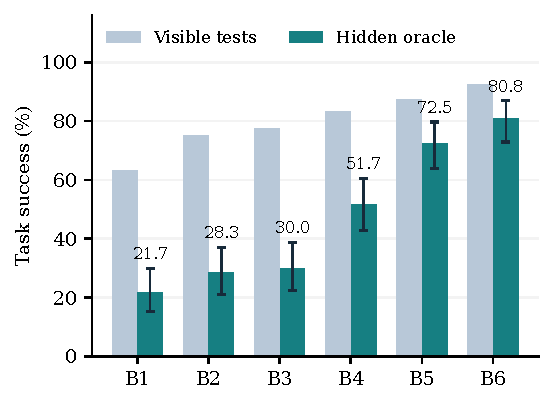
\includegraphics[width=.485\textwidth]{figures/correctness.pdf}\hfill
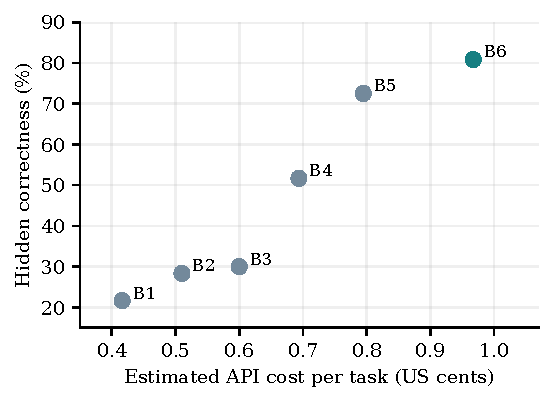
\includegraphics[width=.485\textwidth]{figures/cost_tradeoff.pdf}
\caption{Correctness and resource trade-off. Left: visible and hidden success; error bars are 95\% Wilson intervals for hidden correctness. Right: hidden correctness against estimated API cost per task. B6 has the highest correctness; B5 has the lowest cost per correct repair.}\label{fig:correctness}\label{fig:cost}
\end{figure*}

Pairing reveals overlap that marginal percentages omit. B6 succeeds where B2 fails on 67 tasks, while B2 succeeds where B6 fails on four. Thirty tasks succeed under both and 19 under neither. The difference is 63/120, or 52.5 percentage points, with the reported bootstrap interval [42.5,62.5]. Table~\ref{tab:paired} also compares B6 with B3. B6 therefore does not subsume every baseline success.

\begin{table*}[!t]\centering\small
\caption{Paired hidden-correctness contrasts. Counts are full-only / baseline-only / both / neither. CIs use 20,000 domain-stratified paired bootstrap draws.}\label{tab:paired}
\begin{tabularx}{\textwidth}{@{}lXXr@{}}\toprule
Contrast & Risk difference, pp [95\% CI] & Binary $\delta$ [95\% CI] & Paired counts\\\midrule
B6--B2 & $+52.5$ [42.5,62.5] & .525 [.425,.625] & 67 / 4 / 30 / 19\\
B6--B3 & $+50.8$ [40.8,60.8] & .508 [.408,.608] & 66 / 5 / 31 / 18\\\bottomrule
\end{tabularx}
\end{table*}

\subsection{RQ3: Component ablations}
B3 and B4 differ in contextual representation while retaining test-only feedback. Hidden correctness rises from 36 to 62 tasks, a descriptive gain of 21.7 percentage points. With inferred checks present, changing B5 to B6 raises the count from 87 to 97, a gain of 8.3 points. Adding inferred checks gives 42.5 points in structural context (B5--B3) and 29.2 in SIG context (B6--B4).

Both mechanisms are associated with improved outcomes in this release, but their contributions overlap. The risk-scale interaction is negative: the gain from SIG context is smaller when inferred checks are present. This is consistent with the mechanisms addressing some of the same failures. It neither establishes the cause of an individual success nor justifies treating the gains as additive.

\begin{table}[t]\centering\small
\caption{Descriptive factorial contrasts derived from supplied counts; no additional intervals or significance tests are asserted.}\label{tab:factorial}
\begin{tabularx}{\columnwidth}{@{}Xr@{}}\toprule
Comparison & Difference (pp)\\\midrule
SIG with test-only validation (B4--B3) & $+21.7$\\
SIG with inferred checks (B6--B5) & $+8.3$\\
Checks with AST context (B5--B3) & $+42.5$\\
Checks with SIG context (B6--B4) & $+29.2$\\
Risk-scale interaction & $-13.3$\\\bottomrule
\end{tabularx}
\end{table}

The interaction is $(97-87-62+36)/120=-13.3$ percentage points. Ceiling effects can reduce marginal gains as correctness approaches one, and the richer treatments also use more inference. A budget-matched comparison would help separate those explanations; the present contrasts are descriptive.

B5 includes structural context and B4 retains public tests; neither is a component operating alone. B2 is the test-feedback baseline implemented in this harness, not a reproduction of every test-driven APR system in the literature. These operational definitions matter when transferring conclusions to other tools.

\subsection{RQ4: Financial invariant preservation}
Table~\ref{tab:financial} reports minor-unit, idempotency and routing preservation on 60 banking/payment tasks. B6 preserves all obligations on 52/60 (86.7\%), compared with 19/60 (31.7\%) for B2. Its marginal counts are 56 for minor units, 57 for keys and 58 for routing.

Joint preservation is below each marginal rate because different candidates can violate different obligations. High destination preservation cannot compensate for losing an idempotency key. This financial endpoint is also distinct from whole-benchmark hidden correctness: it covers a task subset and selected assertions.

\begin{table}[t]\centering\small\setlength{\tabcolsep}{3pt}
\caption{Financial preservation ($N=60$). Cells are count (\%).}\label{tab:financial}
\begin{tabular*}{\columnwidth}{@{\extracolsep{\fill}}lrrrr@{}}\toprule
ID & Minor units & Key & Routing & All\\\midrule
B1 & 26 (43.3) & 35 (58.3) & 45 (75.0) & 15 (25.0)\\
B2 & 29 (48.3) & 40 (66.7) & 48 (80.0) & 19 (31.7)\\
B3 & 32 (53.3) & 44 (73.3) & 50 (83.3) & 21 (35.0)\\
B4 & 43 (71.7) & 48 (80.0) & 53 (88.3) & 34 (56.7)\\
B5 & 53 (88.3) & 55 (91.7) & 57 (95.0) & 46 (76.7)\\
B6 & 56 (93.3) & 57 (95.0) & 58 (96.7) & 52 (86.7)\\\bottomrule
\end{tabular*}
\end{table}

\subsection{RQ5: Attempts and estimated API cost}
The summary reports 1.25 mean repair attempts for B6 and 1.60 for B2. Mean prompt tokens increase from 2,600 to 5,400; completion and reasoning tokens increase from 840 to 1,500. B6 thus has higher total estimated API cost: USD 1.1610 across 120 tasks versus USD 0.6120 for B2.

Including failed tasks in the numerator and dividing by hidden successes gives USD 0.01197 per correct repair for B6 and USD 0.01800 for B2, a 33.5\% reduction. The improvement concerns cost per correct result; spending per attempted task increases. B5 has the lowest cost per correct repair (USD 0.01097), while B6 has the highest hidden correctness. Neither dominates both objectives.



Table~\ref{tab:cost} keeps expenditure per task separate from expenditure per correct repair. Figure~\ref{fig:cost} places the correctness gains alongside their API cost.

\ifAccess

The lower ratio for B6 relative to B2 arises because hidden successes increase faster than aggregate cost. Richer context, intent calls and candidate trajectories can all contribute; the aggregate endpoint does not attribute the saving to a particular mechanism.

Token SDs describe dispersion across the supplied records, not repeated invocations of the same task. The release does not value staff time, subscription commitments or production incidents. Its economic result is a token-accounting comparison under explicit fixed rates.
\fi

\section{Discussion}
\subsection{What the visible/hidden gap reveals}
Public tests can establish an endpoint or a nested-object shape while missing the value inside it. The B2 visible rate exceeds its hidden rate by 46.7 percentage points. With inferred checks and SIG context, that gap falls to 11.7 points. The result supports checking relations between inputs and outgoing requests during candidate selection, while retaining an independent endpoint for evaluation.

For an amount, the relevant relation can be exact equality in minor units. For routing, it is the identity supplied by the caller. For an idempotency key, it is preservation of the caller's token across the migration. An assertion that a field exists does not test any of these relations. Showing the asserted relation beside its outcome gives a reviewer a concrete basis for accepting or rejecting a proposal.

\subsection{A failure of inferred-check coverage}
The retained BANK-009/B5 artifact illustrates this gap. Its generated check accepts the endpoint and a populated payload, but the candidate changes the idempotency key and fails the hidden key-preservation assertion. Amount and destination preservation do not compensate for that failure. This is an example of incomplete check inference, not a measured frequency of that defect outside the benchmark.

Other plausible migrations can lose exactness by converting large integers to floating point or place a valid identifier in the wrong route. These mechanisms explain why shape checks need behavioral predicates. The financial table reports the observed preservation outcomes; it does not provide a causal classification of every failed repair.

\ifAccess
\subsection{From an intent statement to an assertion}
Let $p_n$ be the updated path, $b$ a nested transfer object and $k$ the outgoing idempotency key. The BANK-009/B5 structural check can be summarized as
\begin{equation}
T_s(d,o)=[o.path=p_n]\land[\operatorname{isdict}(b)]\land[|b|\ge2].
\end{equation}
The preservation obligation is $R_k(d,o)=[o.k=d.k]$. Since $T_s$ contains no relation between the outgoing key and the input, its passage supplies no evidence for $R_k$. A natural-language rule mentioning idempotency is insufficient when its executable assertion omits that relation.

An obligation-to-assertion review should identify the input, output and relation exercised by each check. Numeric checks should distinguish type, unit and equality; routing checks should identify which destination field is preserved. One possible extension is a metamorphic check that changes the input key while holding other inputs fixed and requires the outgoing key to change accordingly. This extension has not been evaluated, and overly restrictive assertions could reject legitimate migrations.

The same reasoning applies to missing information. If a revised contract requires a currency or billing address absent from the caller's inputs, a plausible default can conceal an unresolved requirement. The engine can return a missing-information diagnostic. Diagnostic quality would need its own evaluator; hidden correctness in this study does not measure it.

\subsection{Review and source freshness}
An acceptance result belongs to the source checkpoint that was tested. Editing the repository or a requirement definition changes the context to which that result applies. The application checks freshness before applying a patch and records individual requirement outcomes. A skipped or erroneous check remains unresolved even if another suite passes.

The interface exposes public tests, inferred checks and confirmed requirements separately. This supports inspection of partial outcomes, but the present study does not measure reviewer effort or usability. A maintainer study could test whether these evidence links improve decisions while controlling task difficulty.
\fi

\subsection{Choosing a repair configuration}
B6 has the highest hidden correctness, whereas B5 has the lowest estimated cost per correct repair. A configuration choice therefore depends on the value placed on additional successful migrations. The experiment uses an unweighted task denominator and does not estimate the business cost of a failed integration or staff time saved by a patch.

The ablation suggests overlapping benefits from SIG context and inferred checks. It does not establish which mechanism caused a particular success. A budget-matched experiment could test whether additional calls alone explain part of the gain. An adaptive policy that expands context after failed checks is another possible study; its effectiveness cannot be inferred from the fixed treatments.

\section{Threats to Validity}
\subsection{Construct validity}
Hidden correctness is bounded by the oracle and its inputs. Financial fixtures assess request-level obligations, including exact amounts, keys and routes; they do not establish remote settlement or exactly-once execution. Generated checks can omit values, duplicate public assertions or encode an incorrect inference. Localization depends on exact-match call-site annotations and the selected distractors.

\subsection{Internal validity and provenance}
The analysis uses the author-supplied evaluation release. Its interpretation depends on correspondence between the reported outcomes and the source, prompts, generated checks and original responses used during execution. Retrospective edits require a separately identified reevaluation; checksums establish byte identity, not execution history. The authors confirm that the reported results correspond to the retained execution records.

Pairing controls task identity, but richer context and auxiliary calls alter inference opportunity. The API model is not an independently established immutable checkpoint. Temperature and seed settings do not guarantee regeneration across service changes. With one realization per task and treatment, repeated-inference variance remains unmeasured.

\subsection{Statistical and external validity}
The intervals describe task-resampling uncertainty conditional on the recorded realization. Shared templates or repository families can induce dependence beyond the domain stratification. Factorial contrasts are descriptive, and multiple endpoints are not independent confirmations of the same effect.

The benchmark consists of authored Python request-builder fixtures. Explicit obligations aid controlled comparison, but transfer to large applications, dynamic SDKs, other languages and naturally occurring migrations requires further evaluation. Estimated API cost depends on the included usage and fixed rate scenario; it excludes caching, infrastructure and staff costs. Trusted-fixture execution also does not evaluate adversarial repository isolation.

\ifAccess
\section{Reproducibility}
\subsection{Task and execution records}
Each public fixture contains client source, old and new contracts, inputs and public checks. Private evaluator assets contain hidden inputs, an oracle and a reference patch. Run evidence links the selected patch to prompts, intermediate candidates, public outcomes, private outcomes and model-call records. The traceability index identifies the task and treatment associated with those assets.

A reproducible release must retain the exact source and selection-time checks. Changing an assertion changes the evaluator definition even if its file name stays the same. A documented export or redaction procedure can protect credentials while preserving the connection between original responses and selected candidates. Text normalization and physical-file hashes should identify their respective representations.

\subsection{Three reproduction operations}
Offline analysis reads the 720-row primary matrix and the 360-row financial matrix to reconstruct summaries. Candidate replay evaluates saved patches against identified fixtures and checks. Model regeneration requests new candidates and produces another inference realization. These operations have different dependencies and costs; arithmetic agreement alone does not establish execution replay or model repeatability.

Tokens should remain separate from the pricing scenario so that future analyses can apply alternative rates without repeating inference. Intermediate attempts and unsuccessful tasks belong in the release alongside successful examples. They establish the denominator for correctness and failure-inclusive expenditure.

\fi

\section{Conclusion}
APIShield combines contract differences, source context and executable preservation checks to produce reviewable REST migration proposals. Across the 120-task evaluation release, B6 achieves 80.8\% hidden correctness versus 28.3\% for iterative test feedback, a paired gain of 52.5 percentage points. It preserves all financial obligations on 52/60 tasks. Its estimated API cost per correct repair is 33.5\% below B2, while B5 achieves the lowest ratio overall. The next evaluation should match inference budgets and test repeated realizations on broader, naturally occurring migrations.


\IEEEtriggeratref{12}
\bibliographystyle{IEEEtran}
\bibliography{../shared/references}
\EOD
\end{document}
